% !TeX spellcheck = it_IT
\newpage
\section{Concept learning}
Il concept learning si tratta di inferire una \textbf{funzione booleana} a partire da esempi positivi o negativi.
\begin{definition}[Esempio]
	Definiamo come esempio la seguente coppia:
	\begin{equation*}
		<x,c(x)> \in D
	\end{equation*}
\end{definition}
\begin{definition}[Soddisfa]
	Una funzione $h:X\to\{0,1\}$ soddisfa $x$ se
	\begin{equation*}
		h(x)=1
	\end{equation*}
\end{definition}
\begin{definition}[Consistenza]
	Un'ipotesi $h$ è consistente con:
	\begin{itemize}
		\item un \textbf{esempio} $<x,c(x)> \quad x \in X$ se $h(x) = c(x)$
		\item un \textbf{insieme di esempi} $D$ se $\forall <x,c(x)> \in D \Longrightarrow h(x) = c(x)$
	\end{itemize}
\end{definition}
\begin{definition}[Problema mal posto]
	Un problema si dice mal posto quando viola:
	\begin{itemize}
		\item L'\textbf{esistenza}
		\item L'\textbf{unicità}
		\item La \textbf{stabilità}
	\end{itemize}
	della soluzione.
\end{definition}
\begin{definition}[Spazio delle ipotesi]
	Dati $n$ input binari, lo spazio delle ipotesi è:
	\begin{equation}
		\lvert H \rvert = 2^{\#-instances}=2^{2^n}
	\end{equation}
\end{definition}
\begin{example}[Funzioni booleane]
	Dati dei valori booleani in input di cui sappiamo l'output, dobbiamo determinare la funzione booleana.
	\begin{table}[!h]
		\centering
		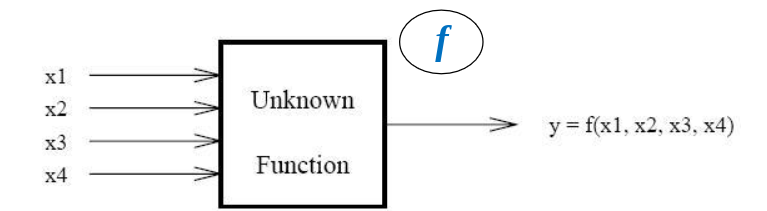
\includegraphics[scale=0.3]{boolean_function.png}
		\begin{tabular}{cccc|c}
			$x_1$ & $x_2$ & $x_3$ & $x_4$ & y \\
			\hline
			0 & 0 & 1 & 0 & 0 \\
			0 & 1 & 0 & 0 & 0 \\
			0 & 0 & 1 & 1 & 1 \\
			1 & 0 & 0  &1 & 1 \\
			0 & 1 & 1 & 0 & 0 \\
			1 & 1 & 0 & 0 & 0 \\
			0 & 1 & 0 & 1 & 0 \\
			\hline
		\end{tabular}
	\end{table}
	\\Questo è una problema \textbf{mal posto} in quanto ci sono più funzioni che potrebbero dare questo risultato (\textbf{unicità}).
	Dati quattro input binari, abbiamo $2^{2^4}= 65536 $ possibili funzioni che dobbiamo esplorare interamente per trovare quella corretta.\\
	È necessario lavorare con uno spazio ristretto di ipotesi $H$.
\end{example}
\begin{definition}[Lookup table]
	Un possibile modello di ML è quello di \textit{Lookup Table}, dove l'algoritmo sa a memoria le risposte che gli sono state date in ingresso e sa rispondere solo se gli viene chiesta una di quelle.
\end{definition}
\subsection{Conjective Rules}
Tramite il costrutto \textbf{AND} possiamo ridurre lo spazio delle ipotesi. Considerando dei letterali $l_i$ come pezzo di una stringa di lunghezza $n$, abbiamo:
\begin{itemize}
	\item Letterali \textbf{positivi} (e.g. $h_1=l_2$, $h2=l_1 \land l_2$, $h_3=true$): $\lvert H \rvert = 2^n$
	\item Letterali anche \textbf{negativi} (e.g. $not(l_i)$): $\lvert H \rvert = 3^n + 1$
\end{itemize}

\begin{example}[Enjoy sport]
	\label{example:enjoy_sport}
	Supponiamo di avere determinati \textbf{attributi} relativi al tempo meteorologico e in corrispondenza se una persona vuole o meno fare sport.\\
	Abbiamo quindi $X$ \textbf{istanze}, una \textbf{funzione obiettivo} ($c:EnjoySport \: X \to \{0,1\}$) e un \textbf{training set} $l$ composto da coppie di tipo $<x_n,c(x_l)$
	\begin{table}[!h]
		\centering
		\begin{tabular}{|ccccccc|}
			\hline
			Sky & Temp & Humid & Wind & Water & Forecast & Enjoy \\
			\hline
			Sunny & Warm & Normal & Strong & Warm & Same & Yes \\
			Sunny & Warm & High & Strong & Warm & Same & Yes \\
			Rainy & Cold & High & Strong & Warm & Change & No \\
			Sunny & Warm & High & Strong & Cool & Change & Yes \\
			\hline
		\end{tabular}
	\end{table}
	\\Rappresentiamo ogni \textbf{ipotesi} come insieme di vincoli sugli attributi scelto tra:
	\begin{itemize}
		\item Un valore specifico, e.g. $Water=Warm$
		\item Un valore che non ci interessa, e.g. $Water=?$
		\item Nessun valore permesso (ipotesi nulla), e.g. $Water=\emptyset$
	\end{itemize}
	Una possibile \textit{ipotesi} (per cui quindi una persona va a fare sport) è la seguente:
	\begin{equation*}
		Sky=Sunny \land Wind=Strong \land Forecast=Same
	\end{equation*}
	L'ipotesi più specifica avrà tutti valori \textit{nulli} mentre quella più generale avrà tutti valori che non ci interessano.\\
	L'\textbf{obiettivo} è quello di trovare un'ipotesi $h$ tale che $h(x)=c(x) \forall x \in X$.
	\begin{note}
		Per ora assumiamo che ogni ipotesi che approssimi la funzione obiettivo correttamente sui training examples, approssimerà anche la funzione sugli esempi non osservati. In generale uno dei problemi fondamentali del ML è la differenza tra analisi teorica ed empirica.
	\end{note}
	Per questo esempio abbiamo
	\begin{equation*}
		3 \cdot 2 \cdot 2 \cdot 2 \cdot 2 \cdot 2 = 96
	\end{equation*}
	istanze distinte e $2^{96}$ \textbf{funzioni possibili}. Possiamo semplificare prendendo le ipotesi \textit{sintatticamente} distinte, ovvero $5\cdot 4 \cdot 4 \cdot4 \cdot 4 \cdot 4 = 5120$, oppure quelle \textit{semanticamente} distinte, ovvero $1+4\cdot3\cdot3\cdot3\cdot3\cdot3 = 973$.
\end{example}

\begin{definition}[Più generale]
	Siano $h_j$ e $h_k$ funzioni booleane definite su $X$. $h_j$ è più generale o uguale di $h_k$ se e solo se:
	\begin{equation}
		\forall x \in X : [(h_k(x) = 1) \to (h_j(x)=1)]
	\end{equation}
\end{definition}
In questo modo possiamo imporre un ordinamento sulle \textit{ipotesi}, del tipo $l_i : l_1 \geq (l_1 \land l_2)$, e strutturarne lo spazio dalle più specifiche alle più generali.
\begin{center}
	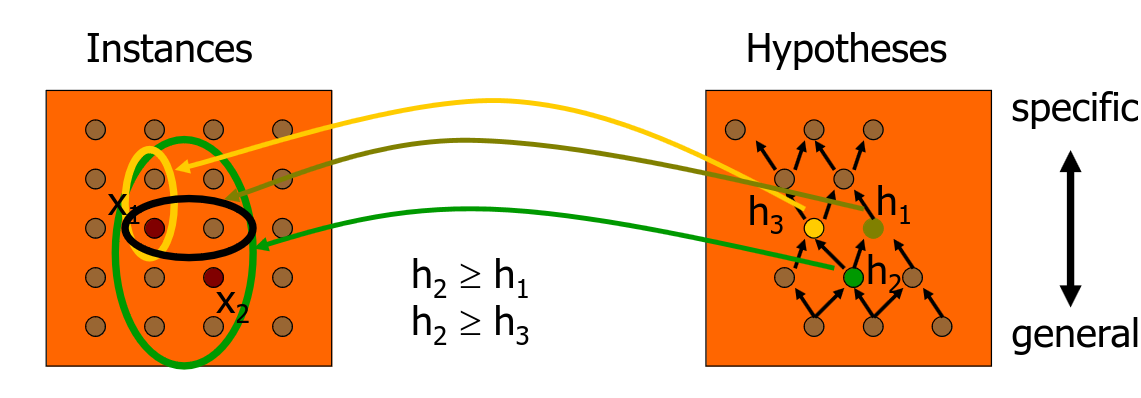
\includegraphics[scale=0.3]{hyp_ordin.png}
\end{center}
\subsubsection{Find-S}
Un algoritmo per cercare una soluzione prevede di ordinare le ipotesi e cercare la più specifica senza bisogno di enumerarle tutte:
\begin{enumerate}
	\item Inizializza $h$ all'ipotesi più specifica in $H$
	\item Per ogni training istance $x$ \textbf{positiva}:
	\begin{lstlisting}
		for each attribute a[i] in h
		if a[i] in h is statisfied by x
		do nothing
		else
		replace a[i] in h by the next more general costraint satisfied by x
	\end{lstlisting}
	\item Restituisci l'ipotesi $h$
\end{enumerate}
\begin{example}
	Partendo dall'esempio \ref{example:enjoy_sport}, facciamo i seguenti passi:
	\begin{enumerate}
		\item $h_0=<\emptyset,\emptyset,\emptyset,\emptyset,\emptyset>$ è la prima ipotesi
		\item Non soddisfa $x_1$. Mettiamo tutti gli attributi in modo che soddisfino al minimo $x_1$. Otteniamo $h_1=<Sunny,Warm,Normal,Strong,Warm,Same>$
		\item $h_1$ non soddisfa $x_2$. Per soddisfarla generalizziamo ulteriormente l'attributo $Humid$, ottenendo $h_2=<Sunny,Warm,?,Strong,Warm,Same>$
		\item $x_3$ è negativa, quindi non la consideriamo
		\item $h_2$ non soddisfa $x_4$. Generalizziamo gli attributi $Water$ e $Forecast$ e otteniamo \\$h_3=<Sunny,Warm,?,Strong,?,?>$
	\end{enumerate}
\end{example}
Questo algoritmo permette di trovare l'ipotesi più specifica che sia consistente con il training example (anche per gli esempi negativi).\\
Un problema è che non c'è \textbf{tolleranza al rumore}, ovvero che non valutando gli esempi negativi non sappiamo se ci sono delle contraddizioni. Inoltre trova solo una soluzione.

\subsubsection{List-Then-Eliminate}
L'idea è di ottenere una descrizione dell'insieme di tutte le ipotesi che siano consistenti con il training example.
\begin{definition}[Version space]
	Il version space $VS_{H,D}$ rispetto allo spazio delle ipotesi $H$ e al training set $D$ è il sottoinsieme delle ipotesi che sono consistenti con tutti i casi del training examples
	\begin{equation}
		VS_{H,D}=\{h \in H \vert Consistent(h,D)\}
	\end{equation}
\end{definition}
L'algoritmo prevede i seguenti passi:
\begin{enumerate}
	\item Faccio una lista di tutte le ipotesi (VersionSpace) $H$
	\item Per ogni training example $<x,c(x)$ rimuovo ogni ipotesi del VS che è inconsistente con quell'esempio
	\item Restituisco il VS
\end{enumerate}
È un algoritmo irrealistico in quanto dovremmo enumerare tutte le ipotesi.
\subsubsection{Candidate Elimination}
\label{alg:cand_elim}
Per evitare di enumerare tutte le ipotesi, possiamo definire il Version Space con dei limiti generali e specifici.
\begin{definition}[General boundary]
	Il limite generale $G$ di un version space $VS_{H,D}$ è l'insieme delle ipotesi più generali in $H$ consistenti con $D$.
\end{definition}
\begin{definition}[Specific boundary]
	Il limite specifico $G$ di un version space $VS_{H,D}$ è l'insieme delle ipotesi più specifiche in $H$ consistenti con $D$.
\end{definition}
\begin{theorem}
	Ogni membro del version space si trova tra il \textbf{general} e lo \textbf{specific} boundary.
	\begin{equation}
		VS_{H,D} = \{h \in H \vert (\exists s \in S) (\exists g \in G) (g\geq h \geq s)\}
	\end{equation}
\end{theorem}
L'algoritmo prevede, per ogni training example $d$, dato $G$ l'insieme delle ipotesi più generali e $S$ quello delle ipotesi più specifiche:
\begin{itemize}
	\item Se $d$ è \textbf{positivo}:
	\begin{enumerate}
		\item Rimuovo da $G$ ogni ipotesi che non sia consistente con $d$
		\item Per ogni ipotesi $s$ che non è consistente con $d$:
		\begin{itemize}
			\item Rimuovo $s$ da $S$
			\item Aggiungo a $S$ tuute le ipotesi $h$ sufficientemente generalizzate in modo che $h$ sia consistente con $d$ e che alcuni elementi di $G$ siano più generali di $h$
			\item Rimuovo da $S$ ogni ipotesi che sia più generale di un'altra ipotesi in $S$
		\end{itemize}
	\end{enumerate}
	\item Se $d$ è \textbf{negativo}:
	\begin{enumerate}
		\item Rimuovo da $S$ ogni ipotesi che non sia consistente con $d$
		\item Per ogni ipotesi $g$ che non è consistente con $d$:
		\begin{itemize}
			\item Rimuovo $g$ da $G$
			\item Aggiungo a $G$ tuute le ipotesi $h$ sufficientemente specializzate in modo che $h$ sia consistente con $d$ e che alcuni elementi di $S$ siano più specializzati di $h$
			\item Rimuovo da $G$ ogni ipotesi che sia meno generale di un'altra ipotesi in $G$
		\end{itemize}
	\end{enumerate}
\end{itemize}
Per \textbf{classificare} i nuovi dati, testiamo la loro consistenza con il version space e vediamo con quante delle ipotesi dà risultato positivo o negativo.

\subsubsection{Bias induttivo}
Il version space non può rappresentare le disgiunzioni (e.g. soleggiato O nuvoloso). Per rimuovere il bias possiamo scegliere uno spazio delle ipotesi $H$ che contenga ogni singolo concetto, ovvero tutti i possibili sottoinsiemi di $X$. Se abbiamo ad esempio $\lvert X \rvert=96$ allora ci sono $\lvert P(X)\rvert = 2^{96}$ concetti distinti. \\
Questa generalizzazione, oltre ad aumentare il tempo necessario per la ricerca, impedisce al modello di classificare nuovi esempi che non siano del training set.
\begin{definition}[Unbiased learner]
	Un unbiased learner non è in grado di generalizzare, in quanto ogni istanza non osservata sarà classificata positivamente da metà delle ipotesi e negativamente dall'altra metà. Ci ritroveremmo quindi con una \textbf{Lookup Table}.
\end{definition}
\noindent Le restrizioni che si fanno sono quindi \textbf{necessarie} per potere fare una generalizzazione. È importante quindi caratterizzare il bias utilizzato e capire qual'è il migliore da scegliere.

\begin{definition}[Inductive bias]
	Il bias induttivo di una algoritmo $L$ è ogni minimo insieme di assunzioni $B$ tali che per ogni concetto obiettivo $c$ e il corrispondente training data $D_c$
	\begin{equation}
		(\forall x_i \in X)[B \land D_c \land x_i] \vdash L(x_i, D_c)
	\end{equation}
	In pratica posso trasformarlo in un sistema \textbf{deduttivo}.
\end{definition}
Negli algoritmi visti fin'ora abbiamo trovato i seguenti bias:
\begin{itemize}
	\item \textbf{Lookup table}: nessun bias
	\item \textbf{Find-S}: lo spazio delle ipotesi contiene il target concept e tutte le istanza sono negative a meno che gli esempi positivi non ci dicano il contrario
	\item \textbf{Candidate Elimination}: lo spazio delle ipotesi contiene il target concept (\textbf{language bias})
\end{itemize}

\subsection{Decision tree}
Introduciamo questa tecnica er risolvere la mancanza di flessibilità del concept learning.

\begin{example}[Tennis]
	\label{example:tennis}
	Poniamo di avere i seguenti dati:
	\begin{table}[H]
		\centering
		\begin{tabular}{|c|ccccc|}
			\hline
			\textbf{Day} & \textbf{Outlook} & \textbf{Temperature} & \textbf{Humidity} & \textbf{Wind} & \textbf{PlayTennis} \\
			\hline
			D1 & Sunny & Hot & High & Weak & No \\
			D2 & Sunny & Hot & High & Strong & No \\
			D3 & Overcast & Hot & High & Weak & Yes \\
			D4 & Rain & Mild & High & Weak & Yes \\
			D5 & Rain & Cool & Normal & Weak & Yes \\
			D6 & Rain & Cool & Normal & Strong & No \\
			D7 & Overcast & Cool & Normal & Strong & Yes \\
			D8 & Sunny & Mild & High & Weak & No \\
			D9 & Sunny & Cool & Normal & Weak & Yes \\
			D10 & Rain & Mild & Normal & Weak & Yes \\
			D11 & Sunny & Mild & Normal & Strong & Yes \\
			D12 & Overcast & Mild & High & Strong & Yes \\
			D13 & Overcast & Hot & Normal & Weak & Yes \\
			D14 & Rain & Mild & High & Strong & No \\
			\hline
		\end{tabular}
	\end{table}
	Un possibile \textit{albero di decisione} è il seguente:
	\begin{center}
		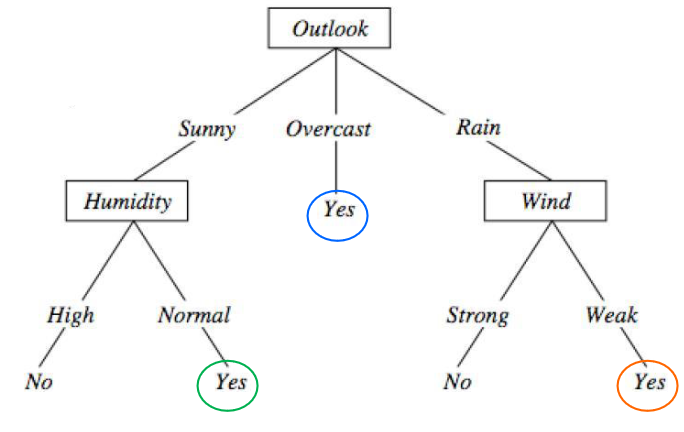
\includegraphics[scale=0.25]{decision_tree_tennis.png}
	\end{center}
	che può anche essere scritto come disgiunzione di congiunzioni:
	\begin{align*}
		& (Outlook=Sunny \land Humidity=Normal) \lor \\
		& (Outlook = Overcast) \lor \\
		& (Outlook=Rain \land Wind=Weak)
	\end{align*}
\end{example}

\subsubsection{ID3}
Dato un insieme di training examples, l'algoritmo fa una ricerca nello spazio degli alberi di decisione e lo costruisce \textbf{top-down} tramite una ricerca \textbf{greedy}. Il punto cruciale è la scelta dell'attributo successivo che possa dare più informazioni. Alla fine, una volta che tutti i casi sono coperti, viene ricostruito ricorsivamente l'albero.
\begin{lstlisting}
	ID3(X: training_ex, T:target_attr, Attrs: other_attr)
	Create Root node
	If all X are +, return Root with class +
	If all X are -, return Root with class -
	If Attrs is empty return Root with class most common value of T in X
	else
	A<- best attribute; decision attribute for Root <- A
	For each possible value v[i] of A:
	- add a new branch below Root, for test A = v[i]
	- X[i] <- subset of X with A = v[i]
	- If X[i] is empty then add a new leaf with class the most common value of T in X
	else add the subtree generated by ID3(X[i], T, Attrs - {A})
	return Root
\end{lstlisting}
Per selezionare il miglior attributo, utilizziamo il concetto di \textbf{entropia}.
\begin{definition}[Entropia]
	L'entropia misura l'impurità di un'insieme di esempi. Dipende dalla distribuzione della variabile casuale $p$.\\
	Dati:
	\begin{itemize}
		\item $S$ un insieme di training examples
		\item $p_+$ la proporzione di esempi positivi in $S$
		\item $p_-$ la proporzione di esempi negativi in $S$
	\end{itemize}
	la definiamo come
	\begin{equation}
		Entropy(S)=-p_+\log_2p_+ - p_-\log_2p_-
	\end{equation}
	Si noti che $0 \leq p \leq 1$ e $0 \leq Entropy \leq 1$
\end{definition}

\begin{definition}[Information gain]
	È la riduzione aspettata dell'entropia causata dal partizionamento degli esempi in base ad un determinato attributo $A$.
	\begin{equation}
		Gain(S,A) = Entropy(S) - \sum_{v \in Values(A)} \frac{\lvert S v \rvert}{\lvert S \rvert} Entropy(Sv)
	\end{equation}
	dove $Sv$ è il sottoinsieme di $S$ per cui $A$ assume valore $v$.
\end{definition}
Più è alto l'\textit{information gain} e più è efficace quel determinato attributo nel classificare i dati. Ci servono quindi degli attributi \textbf{omogenei} (ad esempio totalmente positivi o totalmente negativi). Dobbiamo quindi trovare un attributo $A$ che \textbf{massimizzi} il $Gain$, ovvero con \textbf{bassa} entropia.

\begin{example}
	Partendo dai dati dell'esempio \ref{example:tennis}, calcoliamo prima l'entropia per i vari attributi (9 positivi, 5 negativi):
	\begin{equation*}
		-\frac{9}{14} \log_2(\frac{9}{14}) - \frac{9}{14} \log_2(\frac{9}{14})=0.940
	\end{equation*}
	e poi dei singoli valori che possono assumere, per esempio guardando \textit{Humidity} e \textit{Wind}:
	\begin{itemize}
		\item \textit{Humidity} alta (3 casi positivi e 4 negativi): $-\frac{3}{7} \log_2(\frac{3}{7}) - \frac{4}{7} \log_2(\frac{4}{7})=0.985$
		\item \textit{Humidity} normale (6 casi positivi e 1 negativo): $-\frac{6}{7} \log_2(\frac{6}{7}) - \frac{1}{7} \log_2(\frac{1}{7})=0.592$
		\item \textit{Wind} debole (6 casi positivi e 2 negativi): $-\frac{6}{8} \log_2(\frac{6}{6}) - \frac{2}{8} \log_2(\frac{2}{8})=0.811$
		\item \textit{Wind} forte (3 casi positivi e 3 negativi): $-\frac{3}{6} \log_2(\frac{3}{6}) - \frac{3}{6} \log_2(\frac{3}{6})=1.00$
	\end{itemize}
	Verifichiamo poi il gain dei due attributi selezionati:
	\begin{align*}
		& Gain(S, Humidity) = 0.940 - \frac{7}{14} 0.985 - \frac{7}{14} 0.952 = 0.151 \\
		& Gain(S, Wind) = 0.940 - \frac{8}{14} 0.811 - \frac{6}{14} 1.00 = 0.048
	\end{align*}
	E vediamo che il Gain massimo lo otteniamo scegliendo il parametro Humidity (per cui avevamo trovato un valore minimo di entropia).
\end{example}

\begin{observation}
	L'information gain favorisce gli attributi con tanti possibili valori. Ad esempio nel caso \ref{example:tennis}, la Data avrebbe un gain massimo in quanto ogni giorno corrisponde ad un sottoinsieme puro diverso (quindi 0 entropia). Però non è significativo e utile per generalizzare per istanze nuove.
\end{observation}

\newpage
\noindent Per ovviare a questo problema, introduciamo il Gain Ratio.
\begin{definition}[Gain Ratio]
	Il Gain Ratio si definisce come:
	\begin{equation}
		GainRatio(S,A)=\frac{Gain(S,A)}{SplitInformation(S,A)}
	\end{equation}
	dove, date delle partizioni di $A$ su $v_i$ fino a $c$ valori,
	\begin{equation}
		SplitInformation(S,A)=-\sum_{i=1}^{c}\frac{\lvert S_i \rvert}{\lvert S\rvert} \log_2 \frac{\lvert S_i \rvert}{\lvert S \rvert}
	\end{equation}
	ovvero la misura dell'entropia di $S$ rispetto ai valori di $A$. Più sono uniformemente dispersi i dati e maggiore è il suo valore.
\end{definition}

Adesso il problema è che lo \textit{SplitInformation} può essere $0$ quando $\lvert S_i \rvert \approx \lvert S \rvert$ per un qualche valore $i$. Ovvero quando un attributo ha lo stesso valore per tutti gli esempi. Quindi prima calcoliamo il \textit{Gain} e applichiamo il \textit{GainRatio} solo ai casi che superano una certa soglia.\\
Rispetto al \hyperref[alg:cand_elim]{Candidate Elimination}, adesso:
\begin{itemize}
	\item Lo spazio delle ipotesi è \textbf{completo}
	\item La ricerca mantiene una singola ipotesi corrente
	\item Non c'è backtracking e quindi non c'è la garanzia di ottimalità
	\item Usa tutti gli esempi
	\item Può terminare prima accettando classi imperfette
\end{itemize}

In questo algoritmo il \textbf{bias induttivo} è composto da:
\begin{itemize}
	\item Preferisce alberi più corti a quelli più lunghi
	\item Preferisce alberi che mettono attributi con \textit{Gain} maggiori più vicini alla radice
\end{itemize}
ed è chiamato \textbf{search bias}. Questo è meglio del bias del \textit{Concept Learning} perché non limita la ricerca dall'inizio e permette comunque di avere uno spazio di ricerca ampio.

\begin{definition}[Rasoio di Occam]
	La spiegazione più semplice è più probabilmente la corretta. Nel caso dell'algoritmo ID3, significa di cercare di mantenere un albero più compatto.
\end{definition}

\subsubsection{Overfitting}
\begin{definition}[Overfitting]
	Consideriamo l'errore di un'ipotesi $h$ sia sui dati di training ($error_D(h)$) che su tutti i dati ($error_X(h)$). L'ipotesi $h$ overfitta i dati di training se non esiste un'ipotesi alternativa $h' \in H$ tale che:
	\begin{align*}
		& error_D(h) < error_D(h') \\
		& error_X(h')<error_X(h)
	\end{align*}
\end{definition}
\noindent Nel caso del decision tree:
\begin{center}
	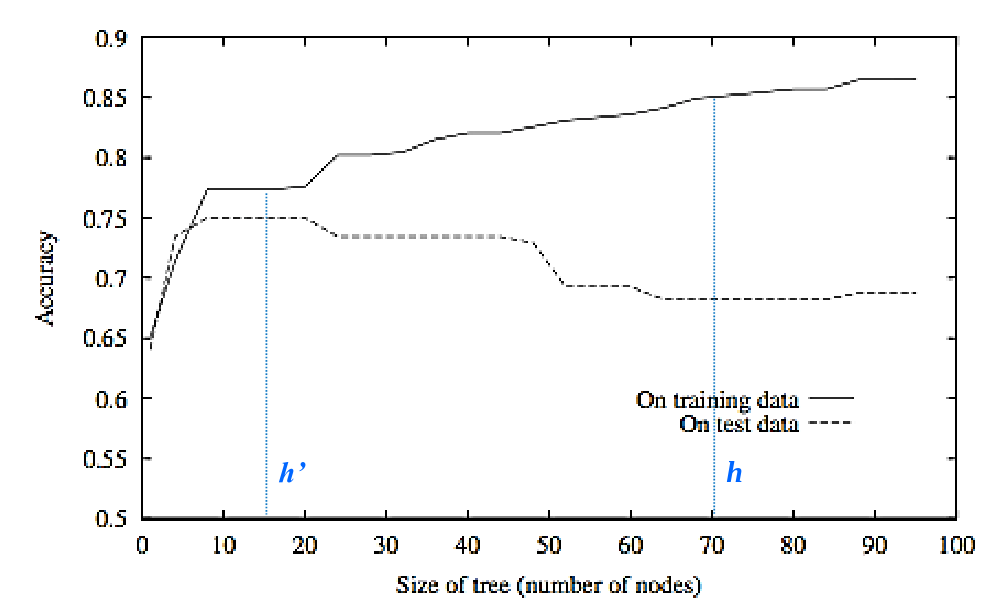
\includegraphics[scale=0.25]{decision_tree_overfitting.png}
\end{center}
Per \textit{attenuarlo}, dobbiamo prima dividere il \textit{training set} in due parti, una per il \textit{training} e l'altra per la \textit{validation}. Poi possiamo scegliere tra due strategie:
\begin{itemize}
	\item \textbf{Early stopping}: bloccare la scelta dell'albero in anticipo, prima della classificazione perfetta
	\item \textbf{Post-prune}: permettere all'albero di fare overfitting e poi tagliarlo successivamente. Il \textbf{pruning} consiste nel rimuovere un sotto albero che ha radice in un nodo: quel nodo diventa una foglia e gli viene assegnata la classificazione più comune. I nodi sono rimossi solo se l'albero che si ottiene non si comporta peggio sul \textit{validation set}. Il \textit{pruning} avviene iterativamente e si ferma quando nessun taglio migliora l'accuratezza.\\
	Un'alternativa più accurata è di dividere l'albero in un insieme di \textbf{regole} e di tagliare quelle che non ne migliorano l'accuratezza. Questa specifica versione migliora anche la \textit{leggibilità}.
	\begin{center}
		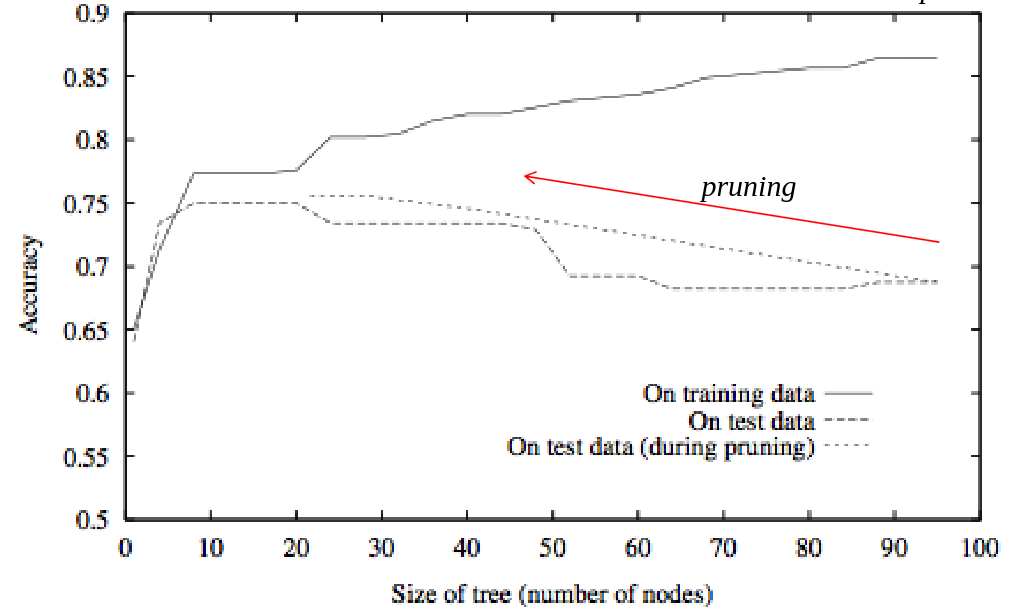
\includegraphics[scale=0.3]{pruning.png}
	\end{center}
\end{itemize}
\subsubsection{Attributi continui}
Potremmo avere invece di attributi concreti, degli attributi continui, ad esempio la temperatura in gradi.\\
Dato un attributo $A$, si crea dinamicamente un nuovo attributo $A_c$ per cui:
\begin{equation*}
	\begin{cases}
		A_c=True & A<c \\
		A_c=False & altrimenti
	\end{cases}
\end{equation*}

\begin{example}
	Se nell'esempio \ref{example:tennis}, l'attributo \textit{Temperature} fosse continuo:
	\begin{table}[H]
		\centering
		\begin{tabular}{|c|cccccc|}
			\hline
			\textbf{Temperature} & 40 & 48 & 60 & 72 & 80 & 90 \\
			\textbf{PlayTennis} & No & No & Yes & Yes & Yes & No \\
			\hline
		\end{tabular}
	\end{table}
	Si determina un \textit{treshold} possibile facendo la media dei valori consecutivi dove c'è un cambio nella classificazione:
	\begin{align*}
		& \frac{48+60}{2} = 54\\
		& \frac{80+90}{2} = 85
	\end{align*}
	E poi si valuta ogni \textit{treshold} in base all'\textit{information gain}, in questo caso $54$.
\end{example}
\subsubsection{Dati incompleti}
Nel caso di un attributo mancante, ad esempio un esame del sangue necessario per una diagnosi, si usa la strategia detta \textbf{imputation}. Questa consiste in varie opzioni:
\begin{enumerate}
	\item Assegno il valore più comune tra gli esempi per il training o nella stessa classe
	\item Assegno una probabilità $p_i$ ad ogni valore $v_i$ basandomi sulle frequenze e assegno i valori mancanti in base alla distribuzione
	\item Classifico un nuovo esempio nello stesso modo (pesato) e la classificazione più probabile viene scelta
\end{enumerate}
\subsubsection{Costi diversi}
Determinati attributi possono avere associati un costo e potremmo voler scegliere alberi che tengano in considerazione attributi meno costosi. Ci sono due possibili modifiche all'algoritmo ID3:
\begin{itemize}
	\item Tan and Schlimmer
	\begin{equation*}
		\frac{Gain^2(S,A)}{Cost(A)}
	\end{equation*}
	\item Nunez
	\begin{equation*}
		\frac{2^{Gain(S,A)-1}}{(Cost(A)+1)^w} \quad\quad w \in [0,1]
	\end{equation*}
\end{itemize}

\subsubsection{Visione geometrica}
Il decision tree divide lo spazio degli input in rettagoli con i lati paralleli agli assi  ed etichetta ognuno di essi con una delle $K$ classi (foglie dell'albero).
\begin{center}
	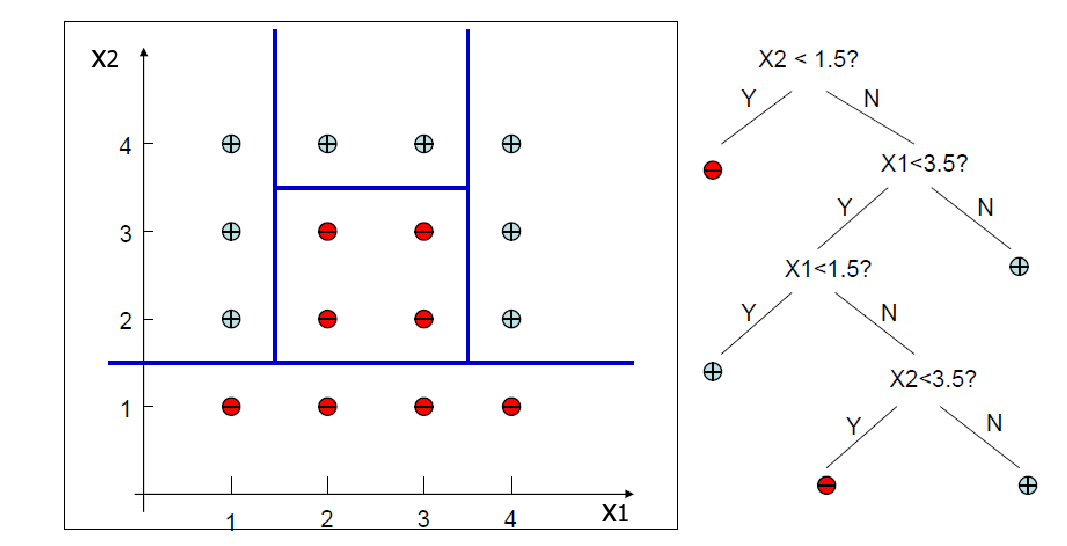
\includegraphics[scale=0.4]{decision_tree_geometry.png}
\end{center}
Si noti come sarebbe sufficiente dare qualche dato che si trovi sul "bordo" del treshold della classificazione per mettere in crisi il decision tree.